\documentclass[border=5pt]{standalone}
\usepackage{tikz}
\usetikzlibrary{shapes, arrows.meta, positioning}

\begin{document}
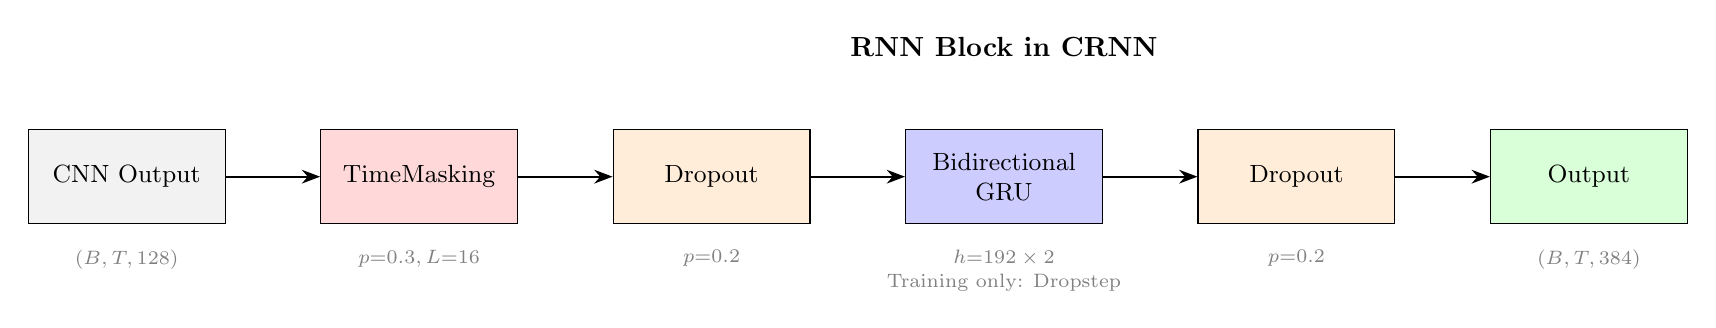
\begin{tikzpicture}[
    node distance=1.2cm,
    >=Stealth,
    block/.style={rectangle, draw, fill=#1, minimum width=2.5cm, minimum height=1.2cm, align=center, font=\small},
    block/.default={white},
    arrow/.style={->, thick},
    dim/.style={font=\scriptsize, text=gray}
]

% 入力
\node[block=gray!10] (input) {CNN Output};
\node[dim, below=0.2cm of input] {$(B, T, 128)$};

% Dropstep
\node[block=red!15, right=of input] (dropstep) {TimeMasking};
\node[dim, below=0.2cm of dropstep] {$p{=}0.3, L{=}16$};

% Dropout (RNN前)
\node[block=orange!15, right=of dropstep] (dropout1) {Dropout};
\node[dim, below=0.2cm of dropout1] {$p{=}0.2$};

% BiGRU
\node[block=blue!20, right=of dropout1] (bigru) {Bidirectional\\GRU};
\node[dim, below=0.2cm of bigru] {$h{=}192 \times 2$};

% Dropout (RNN後)
\node[block=orange!15, right=of bigru] (dropout2) {Dropout};
\node[dim, below=0.2cm of dropout2] {$p{=}0.2$};

% 出力
\node[block=green!15, right=of dropout2] (output) {Output};
\node[dim, below=0.2cm of output] {$(B, T, 384)$};

% 矢印
\draw[arrow] (input) -- (dropstep);
\draw[arrow] (dropstep) -- (dropout1);
\draw[arrow] (dropout1) -- (bigru);
\draw[arrow] (bigru) -- (dropout2);
\draw[arrow] (dropout2) -- (output);

% タイトルと注釈
\node[font=\bfseries, above=0.8cm of bigru] (title) {RNN Block in CRNN};
\node[font=\scriptsize, text=gray, below=0.5cm of bigru] {Training only: Dropstep};

\end{tikzpicture}
\end{document}
